\section{Sistema Operativo Móvil Android}

Android es un sistema operativo y una plataforma software, basado en Linux, que junto con aplicaciones middleware está enfocado para ser utilizado en dispositivos móviles como teléfonos inteligentes, tabletas, google TV y otros dispositivos. Android permite programar en un entorno de trabajo (framework) de Java, lo que nos asegura que podrán ser ejecutadas en cualquier tipo de CPU, tanto presente como futuro. Aplicaciones sobre una máquina virtual Dalvik (una variación de la máquina de Java con compilación en tiempo de ejecución creada por Google optimizada para dispositivos móviles). Además, lo que le diferencia de otros sistemas operativos, es que cualquier persona que sepa programar puede crear nuevas aplicaciones, widgets o incluso, modificar el propio sistema operativo, dado que Android es de código libre. \cite{Android}

\begin{figure}[htbp]
	\centering
		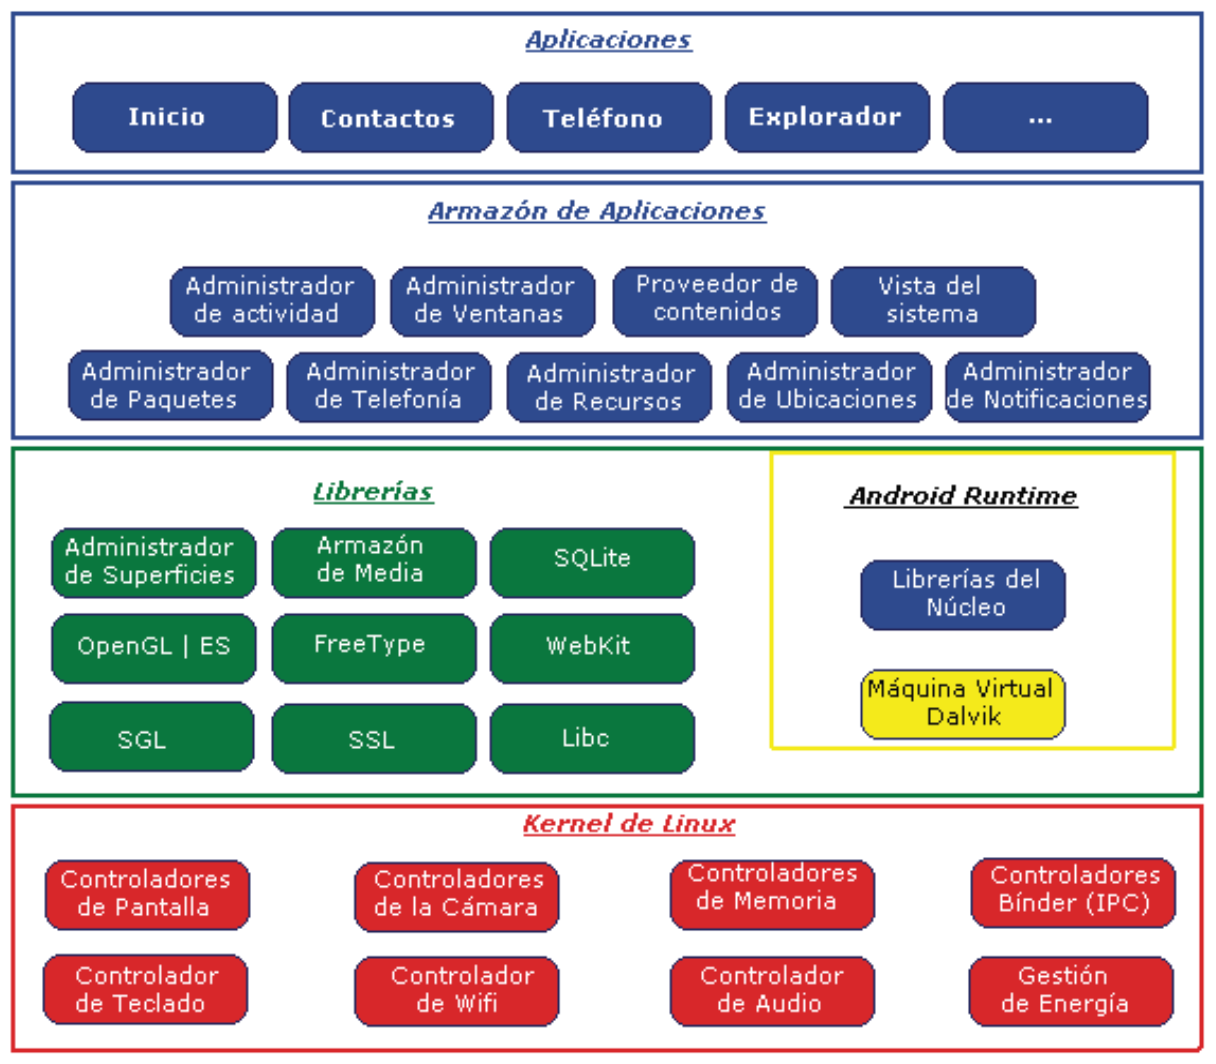
\includegraphics[width=1\textwidth]{Figuras/capasAndroid.png}
		\rule{30em}{0.5pt}
	\caption[Sistema de capas de Android]{Sistema de capas de Android}
	\label{fig:capasAndroid}
\end{figure}

En la Figura \ref{fig:capasAndroid} se distinguen claramente cada una de las capas: la que forma parte del propio Kernel de Linux, donde Android puede acceder a diferentes controladores, las librerías creadas para el desarrollo de aplicaciones Android, la siguiente capa que organiza los diferentes administradores de recursos, y por último, la capa de las aplicaciones a las que tiene acceso.

\begin{itemize}
	\item \textbf{Arquitectura basada en componentes}
	\begin{itemize}
		\item El diseño de la interfaz de usuario se hace en xml, lo que permite que una misma aplicación se ejecute en un dispositivo móvil de pantalla reducida o en un TV.
	\end{itemize}
	\item \textbf{Filosofía de dispositivo siempre conectado a Internet}
	\begin{itemize}
		\item Servicios incorporados basados en Web.
		\item Localización basada tanta en GPS como en redes, bases de datos con SQL, navegadora, multimedia.
	\end{itemize}
	\item \textbf{Aceptable nivel de seguridad}
	\begin{itemize}
		\item Los programas se encuentran aislados unos de otros gracias al concepto de ejecución dentro de una caja que hereda de Linux.
		\item Cada aplicación dispone de una serie de permisos que limitan su rango de actuación (servicios de localización, acceso a Internet, etc.)
	\end{itemize}
	\item \textbf{Calidad de gráficos y sonido}
	\begin{itemize}
		\item Gráficos en 3 dimensiones basados en OpenGL.
		\item Gráficos vectoriales suavizados.
		\item Animaciones inspiradas en Flash.
		\item Incorpora codecs estándar más comunes de audio y vídeo, incluyendo H.264 (AVC), MP3, AAC, etc.
	\end{itemize}
\end{itemize}

\subsection{Características de Android}

\begin{itemize}
	\item \textbf{Acceso a Hardware, incluyendo Cámara, GPS y Sensores: }Android incluye API’s que permite simplificar el desarrollo sin importar el hardware sobre el que se está trabajando. Esto asegura que no necesitamos crear implementaciones específicas para distintos dispositivos, así que podemos crear aplicaciones que deben trabajar según lo esperado en cualquier dispositivo que tenga una versión compatible de Android.
	\item \textbf{Transferencia de Datos con Wi-Fi, BlueTooth y NFC: } Android ofrece soporte muy completo para transferir datos entre dispositivos, incluyendo Bluetooth, Wi-Fi y Android Beam. Estas tecnologías permiten compartir datos entre dispositivos, dependiendo del hardware disponible en el dispositivo utilizado.
	\item \textbf{Mapas y Geolocalización: }El manejo de mapas embebido con el que cuenta Android permite crear aplicaciones que de manera programática pueden manipular los mapas de Google Maps. Además, la integración de un GPS y los servicios de localización de Google para determinar la ubicación actual del dispositivo, permite combinar posicionamiento con mapas.
	\item \textbf{Servicios en Segundo Plano (Background Services): }Android soporta aplicaciones y servicios diseñados para ser ejecutados en segundo plano, mientras nuestra aplicación no está activa, debido a que solamente una aplicación puede estar visible a la vez. 
	\item \textbf{Base de Datos SQLite: }El almacenamiento y la recuperación de información de manera rápida y eficiente es básica para dispositivos con capacidad limitada. Android utiliza SQLite para cumplir con este objetivo. Las aplicaciones móviles pueden aprovechar esta base de datos relacional para almacenar y recuperar información de manera segura y eficiente.
	\item \textbf{Compartición de Datos y Comunicación entre Aplicaciones: }Android incluye técnicas para compartir información entre las distintas aplicaciones, tales como: Intents y Content Providers.
	\item \textbf{ Soporte para gráficos 2D y 3D: }Android provee librerías gráficas para dibujos 2D y 3D con OpenGL. Además, Android provee soporte para imágenes, video, audio, incluyendo video en formato mpeg4.
	\item \textbf{Optimización de Memoria y Administración de Procesos: }Android utiliza su propia maquina virtual para la administración de la memoria. Android asegura que una aplicación responda en un tiempo determinado, de lo contrario la detiene y la puede eliminar en caso de ser necesario, con el objetivo de liberar recursos. De esta manera Android controla el ciclo de vida de las aplicaciones en un ambiente enfocado en hacer más eficiente el uso de memoria de los dispositivos. \cite{presentacionAndroid}
\end{itemize}
